\section{Projektorganisation}

Die Studierenden werden im Projekt 2 (pro2E) für den Studiengang Elektro- und Informationstechnik von fünf Dozenten der Fachhochschule Nordwestschweiz (FHNW) unterstützt. Pascal Buchschacher informiert über Projektmanagement allgemein, Anita Gertiser vermittelt den Studenten die richtige Kommunikation innerhalb des Teams und Peter Niklaus, Richard Gut  wie auch Sebastian Gaulocher steht als Ansprechpartner für Fragen technischer Natur zur Verfügung.

%TODO Die Studierenden werden im Projekt 2 (pro2E) für den Studiengang Elektro- und Informationstechnik von fünf Dozenten der Fachhochschule Nordwestschweiz (FHNW) unterstützt. Pascal Buchschacher betreut das Projektmanagement. Anita Gertiser unterrichtet gleichzeitig Berichtswesen und hilft bei der Kommunikation innerhalb des Teams. Peter Niklaus, Richard Gut und Sebastian Gaulocher stehen als Ansprechpartner für inhaltliche Fragen zur Verfügung.

\subsection{Projektverantwortliche}

\subsection{Auftraggeber}
Auftraggeber des Projekts 2 ist Dr. Luca Dalessandro, Group Technology Manager der Schaffner Group.

\subsection{Teammitglieder}
Das Team 1 des Projekts 2 setzt sich aus sechs Studenten der Fachhochschule Nordwestschweiz, Hochschule für Technik in Brugg/Windisch zusammen. Niklaus Schwegler (NS) ist der Projektleiter und verantwortlich für die Arbeiten und die Kommunikation mit dem Auftraggeber und den Fachdozenten. Unterstützt wird er vom stellvertretenden Projektleiter  Marco  Binder (MB). Für das Ressort Software ist Pascal Puschmann (PP), für das Ressort Elekrotechnik ist Lukas von Däniken (LD) zuständig. Die übrigen Mitglieder sind Simon Rohrer (SR) und Claudio Alfare (CA). 

\subsection{Organigramm}
\begin{figure}[H]
	\centering
	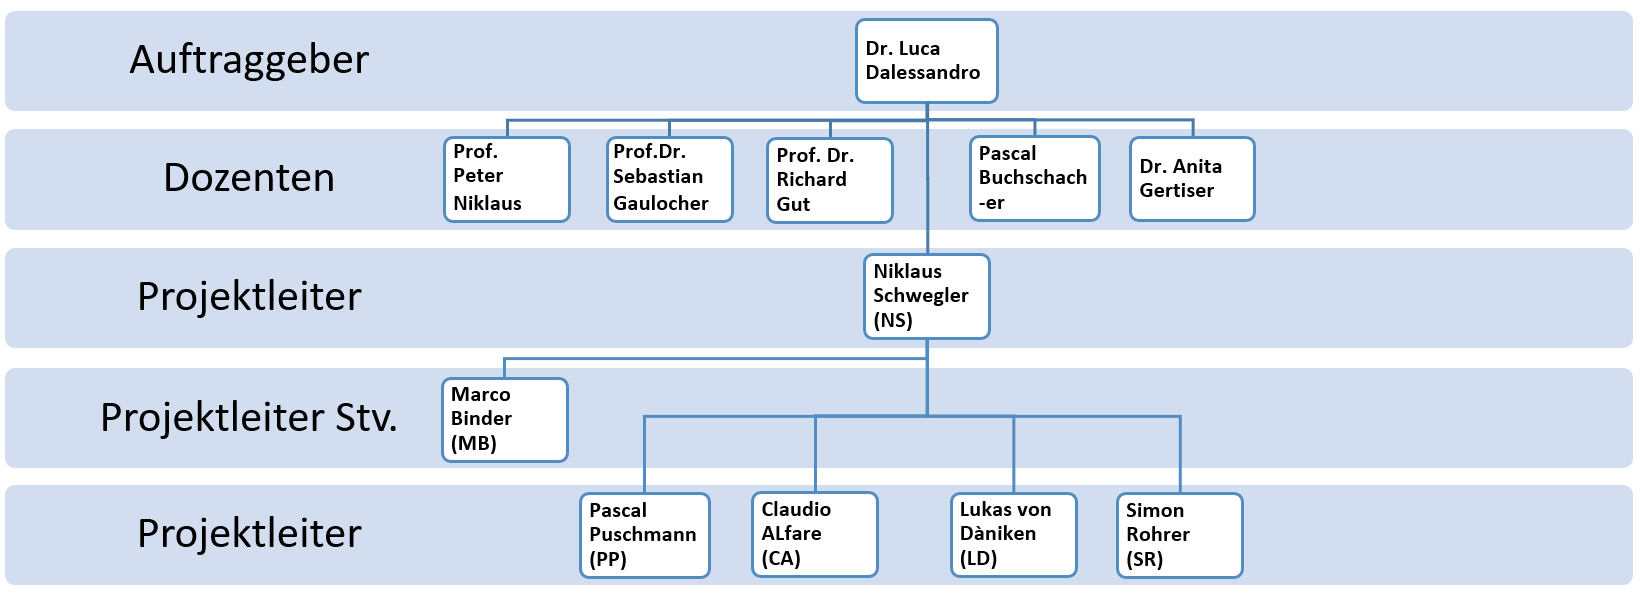
\includegraphics[width=16cm]{Organi.png}
	\label{fig:Organigramm}
\end{figure}
